\documentclass[a4paper]{jsarticle}

%======================================================================
%		論文のタイトル,著者,日付
%======================================================================

\title{\Huge データマイニング工学\\\huge 第1回レポート\vspace{120mm}}
\author{\Large 濱崎 直紀\\\large (学籍番号:28G19096)\vspace{25mm}}
\date{令和2年1月20日}

%======================================================================
%		マクロの読み込みとコマンドの定義
%======================================================================

\usepackage{graphicx}       % eps fileを張り付けるのに必要
% \usepackage[dvipdfmx]{graphicx}     % png等の画像を貼りつけるのに必要
\usepackage{bm}     % 太字を書くのに必要
\usepackage{here}       % その場所に画像を入れるのに必要
% \usepackage{comment}        % コメントを挟むのに必要
% \usepackage{listings}      % ソースコードを表示するのに必要
% \usepackage{jlisting}       % ソースコード内に日本語のコメントアウトがある場合必要(TEX Liveの場合,別途ダウンロードが必要)
\usepackage{caption}

%======================================================================
%		本文
%======================================================================

\begin{document}

\begin{titlepage}
\maketitle
\thispagestyle{empty}
\end{titlepage}

\section*{テーマ}
これからの世界のために考えていること

\subsection*{(回答)}
本文.

\section*{問題2}
\noindent
更新式を
\begin{eqnarray*}
    \left(\begin{array}{c}w_1\\w_2\\w_0\end{array}\right)=\left(\begin{array}{c}w_1\\w_2\\w_0\end{array}\right)+y\left(\begin{array}{c}x_1\\x_2\\-1\end{array}\right)
\end{eqnarray*}
とおくと,更新過程は以下の13ステップとなった.
\begin{table}[H]
    \begin{center}
        \begin{tabular}{c|ccc}
            \hline
            更新回数 & $w_1$ & $w_2$ & $w_0$\\
            \hline \hline
            0 & 1.0 & 1.0 & 0.0\\
            1 & -1.0 & 2.0 & -1.0\\
            2 & 1.0 & 2.1 & 0.0\\
            3 & -1.0 & 2.0 & 1.0\\
            4 & 1.0 & 3.0 & 0.0\\
            5 & -1.0 & 2.9 & 1.0\\
            6 & 1.0 & 3.9 & 0.0\\
            7 & -1.0 & 3.8 & 1.0\\
            8 & 1.0 & 3.9 & 2.0\\
            9 & -1.0 & 3.8 & 3.0\\
            10 & 1.0 & 4.8 & 2.0\\
            11 & -1.0 & 4.7 & 3.0\\
            12 & 1.0 & 5.7 & 2.0\\
            13 & -1.0 & 5.6 & 3.0\\
            \hline
        \end{tabular}
    \end{center}
\end{table}
これを図示すると以下のようになる.
\begin{figure}[H]
    \begin{minipage}{0.3\hsize}
        \begin{center}
            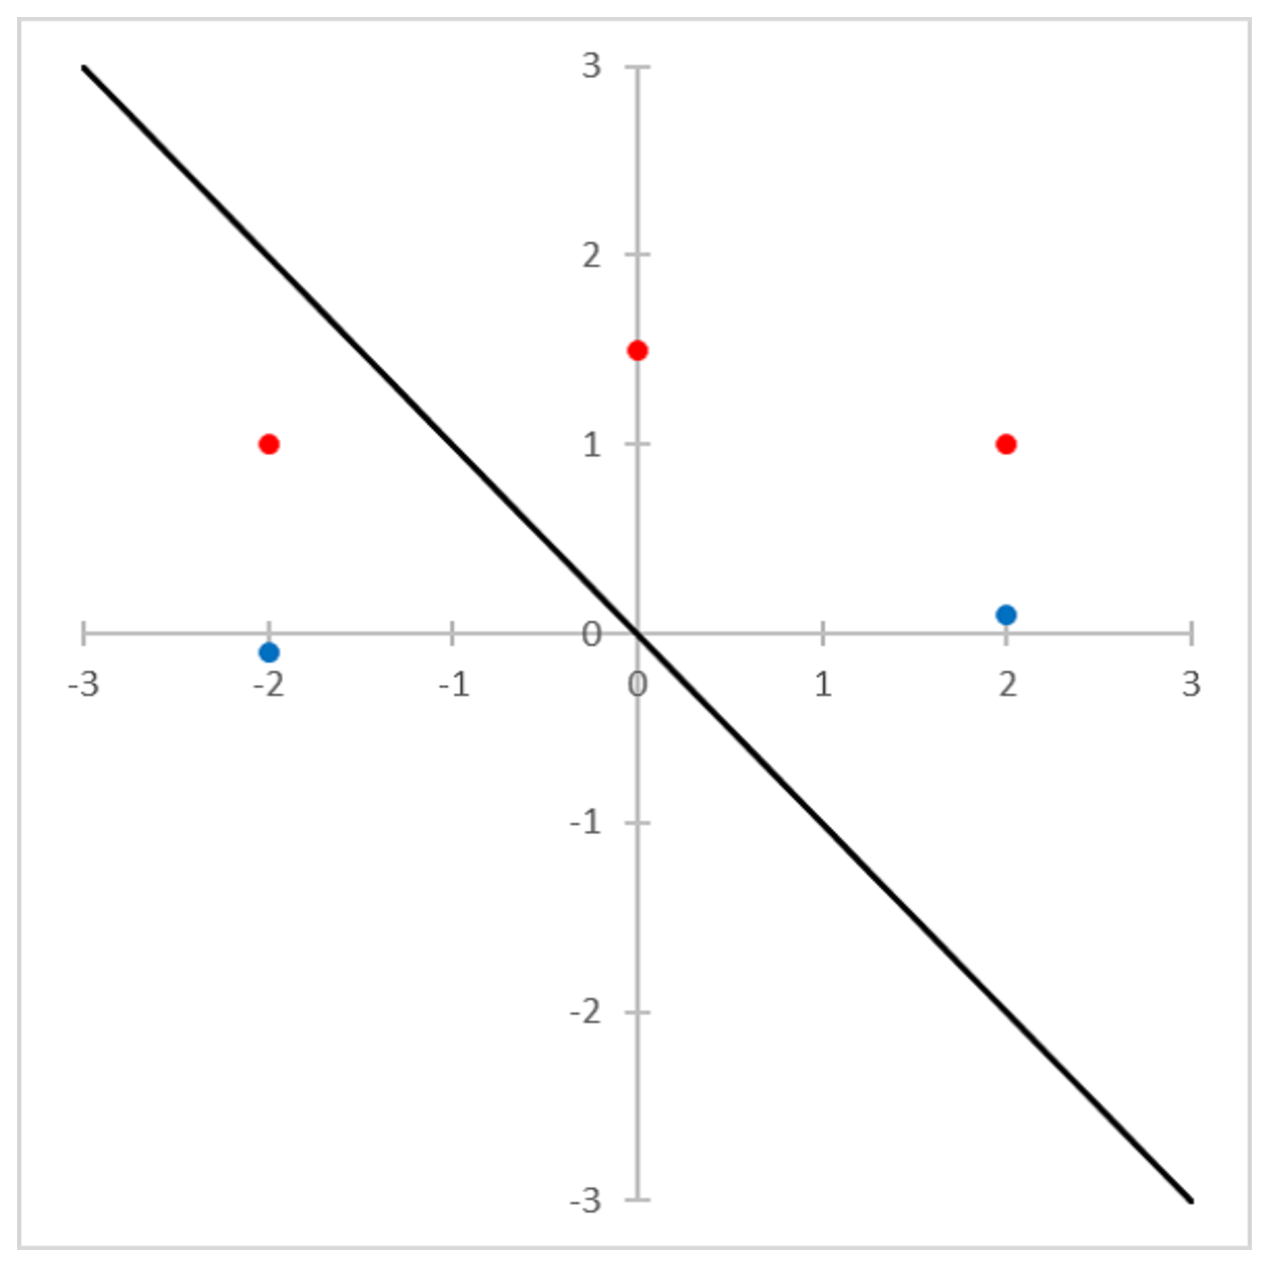
\includegraphics[width=40mm]{./figures/section_2/image0.eps}
            \captionsetup{labelformat=empty,labelsep=none}
            \caption{$w_{(0)}$}
        \end{center}
    \end{minipage}
    \begin{minipage}{0.3\hsize}
        \begin{center}
            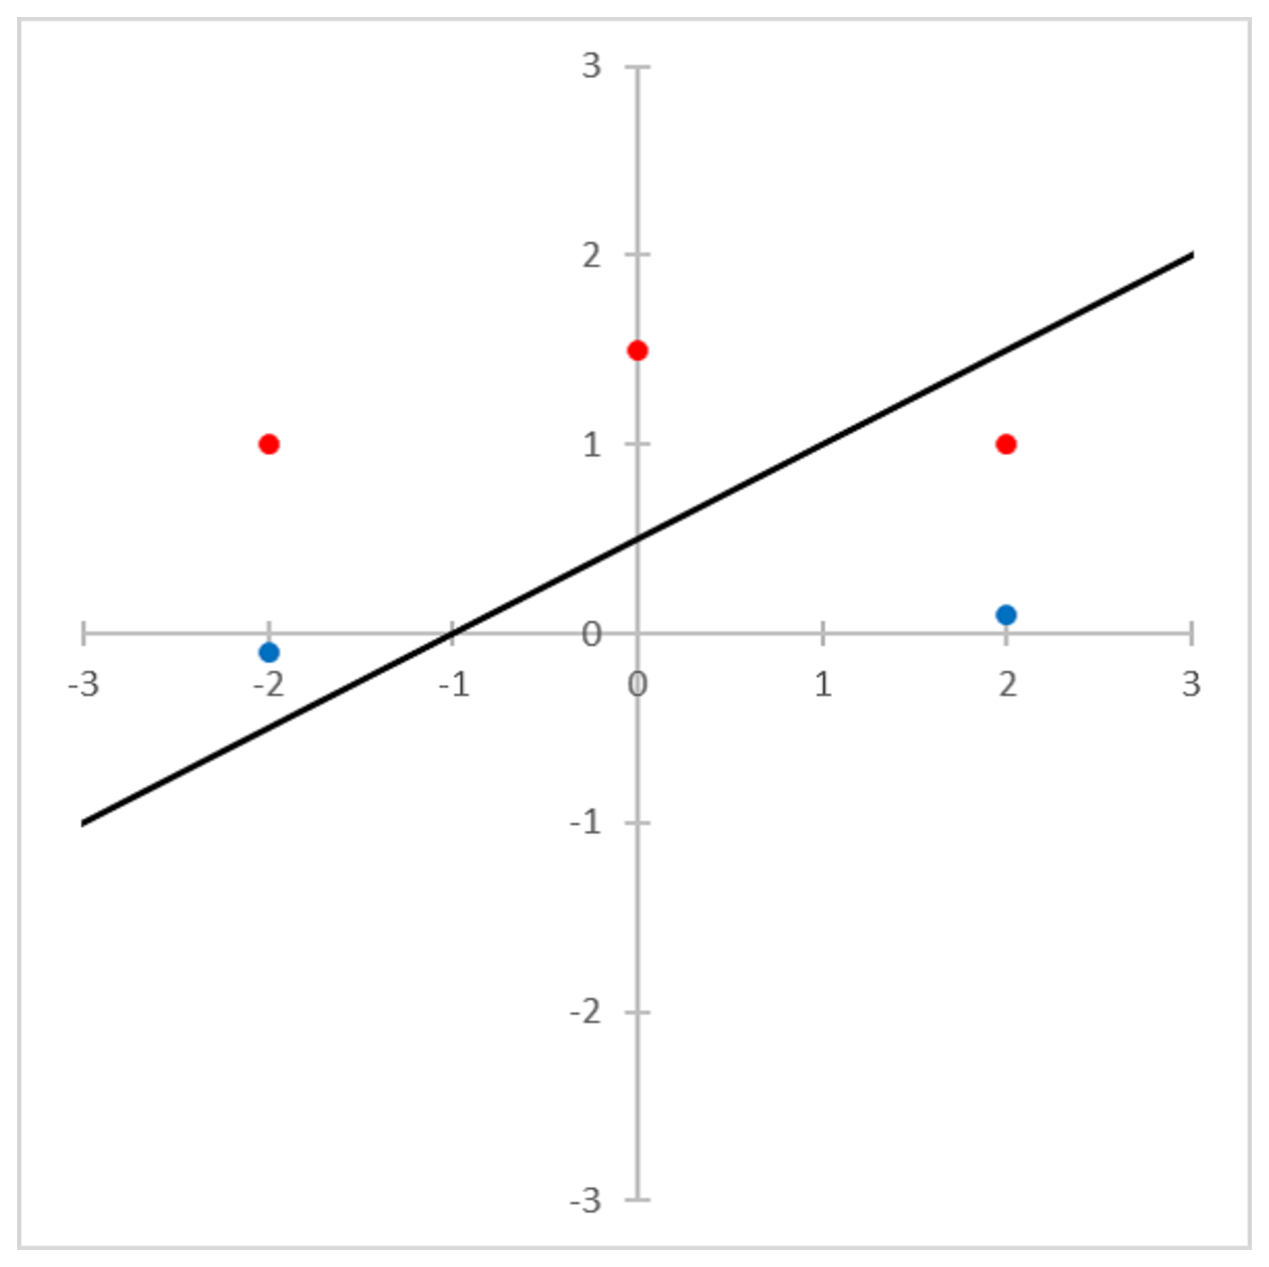
\includegraphics[width=40mm]{./figures/section_2/image1.eps}
            \captionsetup{labelformat=empty,labelsep=none}
            \caption{$w_{(1)}$}
        \end{center}
    \end{minipage}
    \begin{minipage}{0.3\hsize}
        \begin{center}
            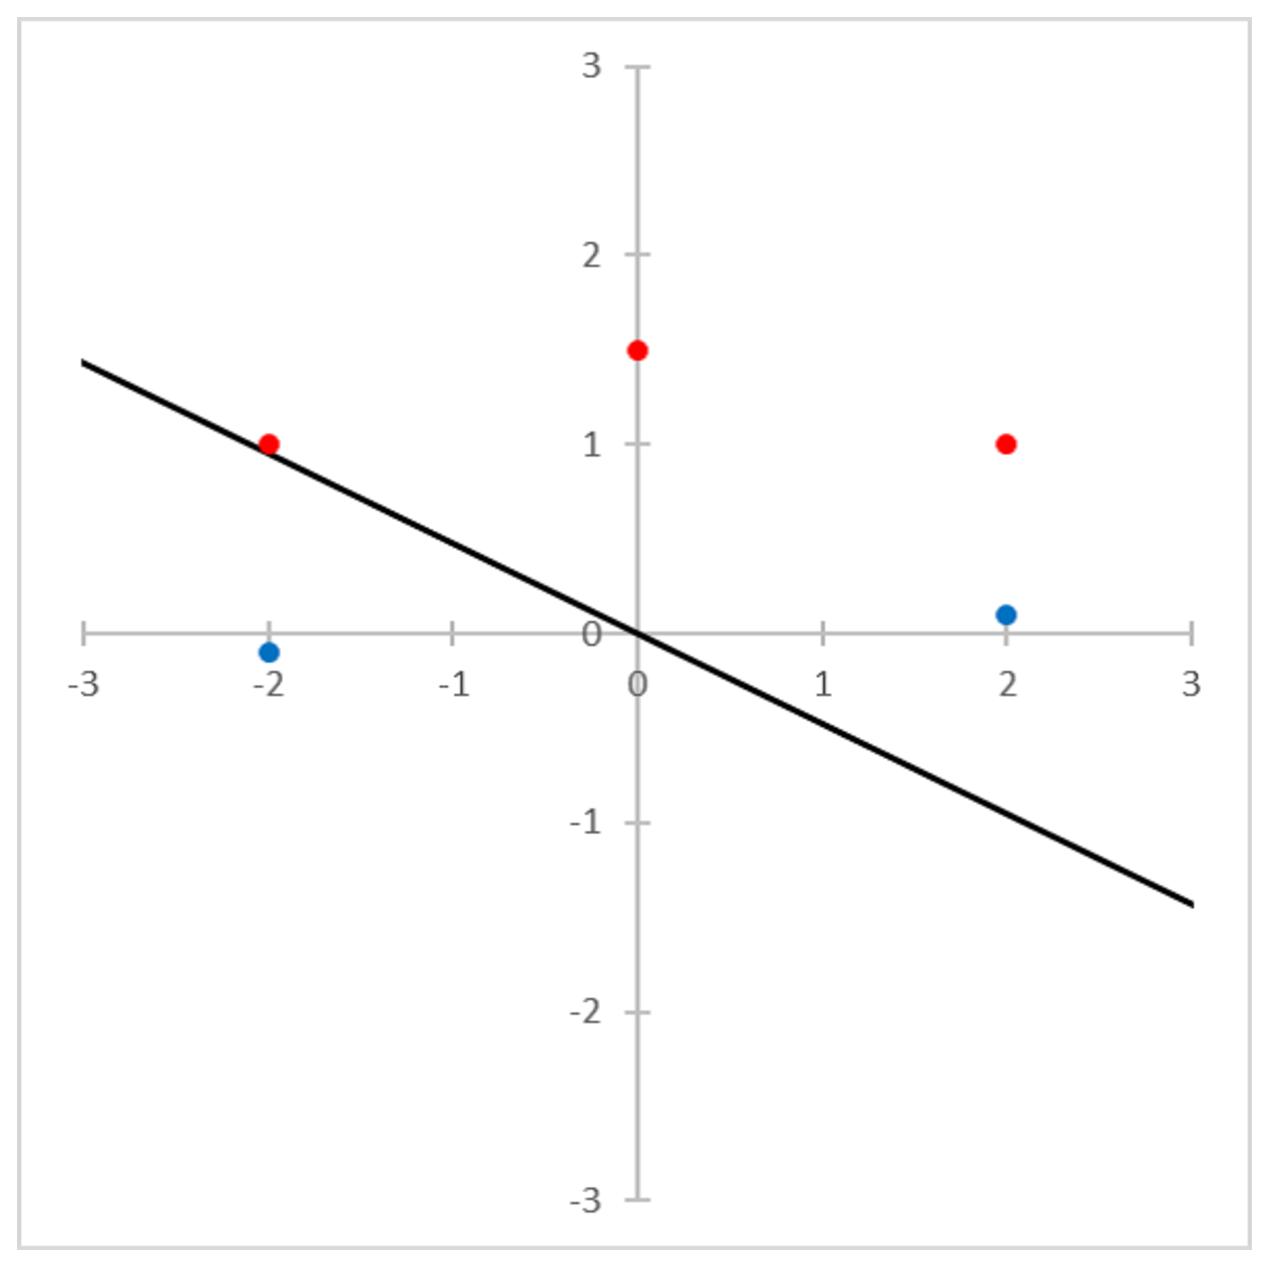
\includegraphics[width=40mm]{./figures/section_2/image2.eps}
            \captionsetup{labelformat=empty,labelsep=none}
            \caption{$w_{(2)}$}
        \end{center}
    \end{minipage}
\end{figure}
\begin{figure}[H]
    \begin{minipage}{0.3\hsize}
        \begin{center}
            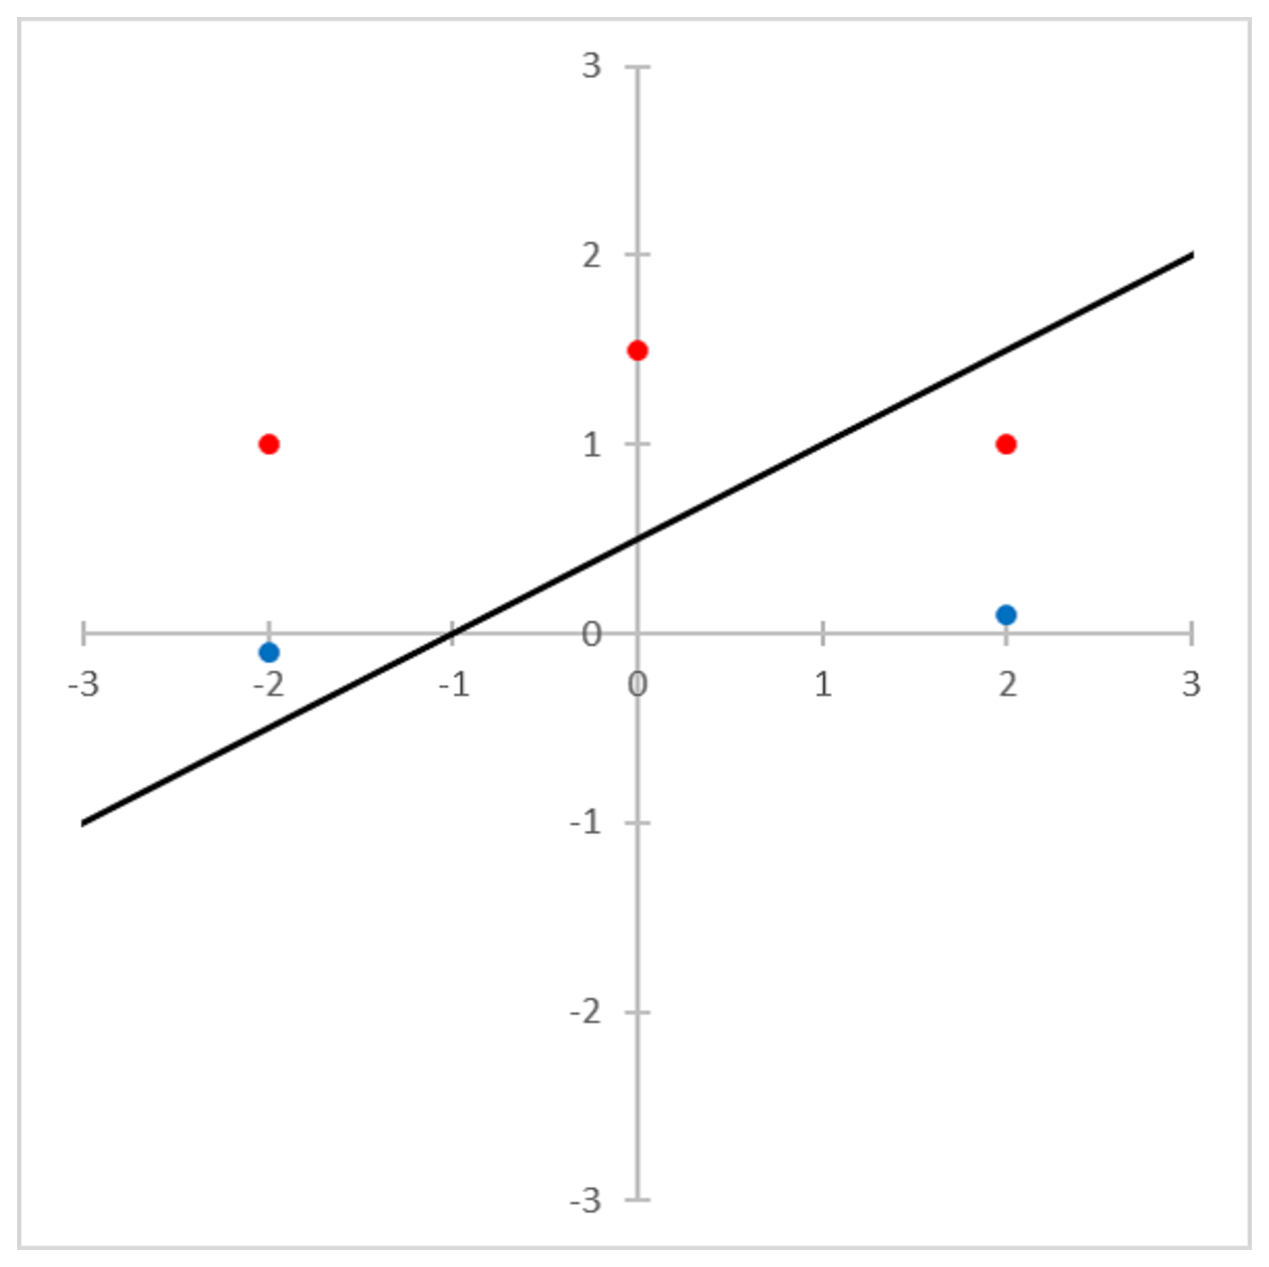
\includegraphics[width=40mm]{./figures/section_2/image3.eps}
            \captionsetup{labelformat=empty,labelsep=none}
            \caption{$w_{(3)}$}
        \end{center}
    \end{minipage}
    \begin{minipage}{0.3\hsize}
        \begin{center}
            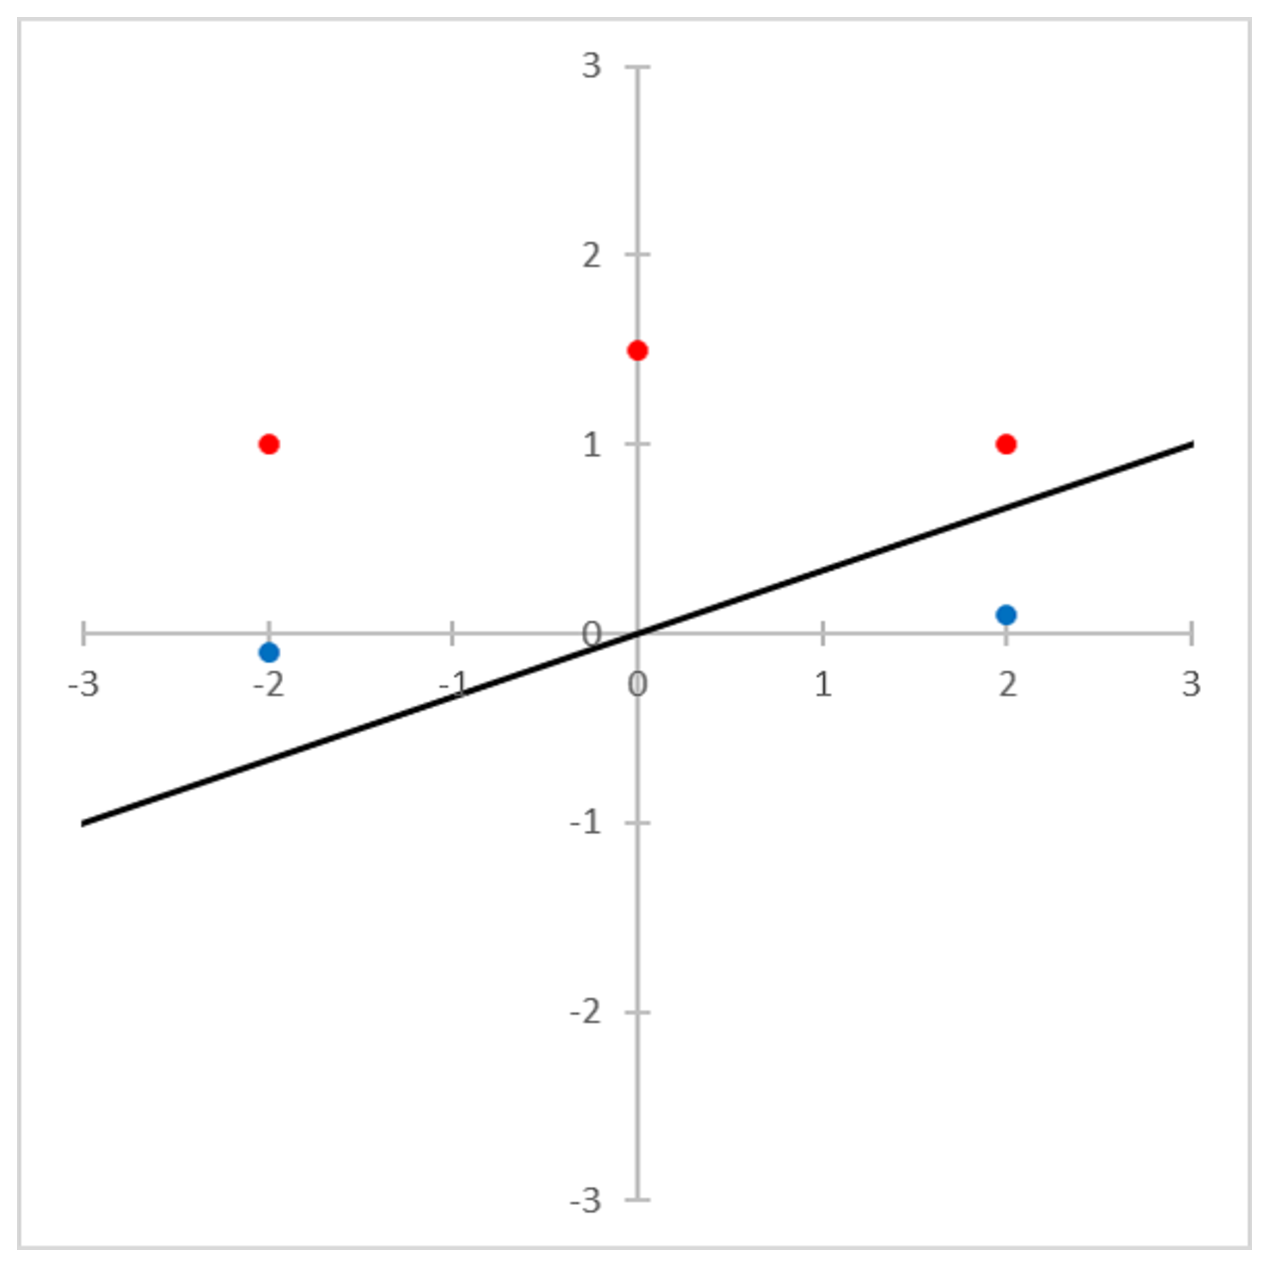
\includegraphics[width=40mm]{./figures/section_2/image4.eps}
            \captionsetup{labelformat=empty,labelsep=none}
            \caption{$w_{(4)}$}
        \end{center}
    \end{minipage}
    \begin{minipage}{0.3\hsize}
        \begin{center}
            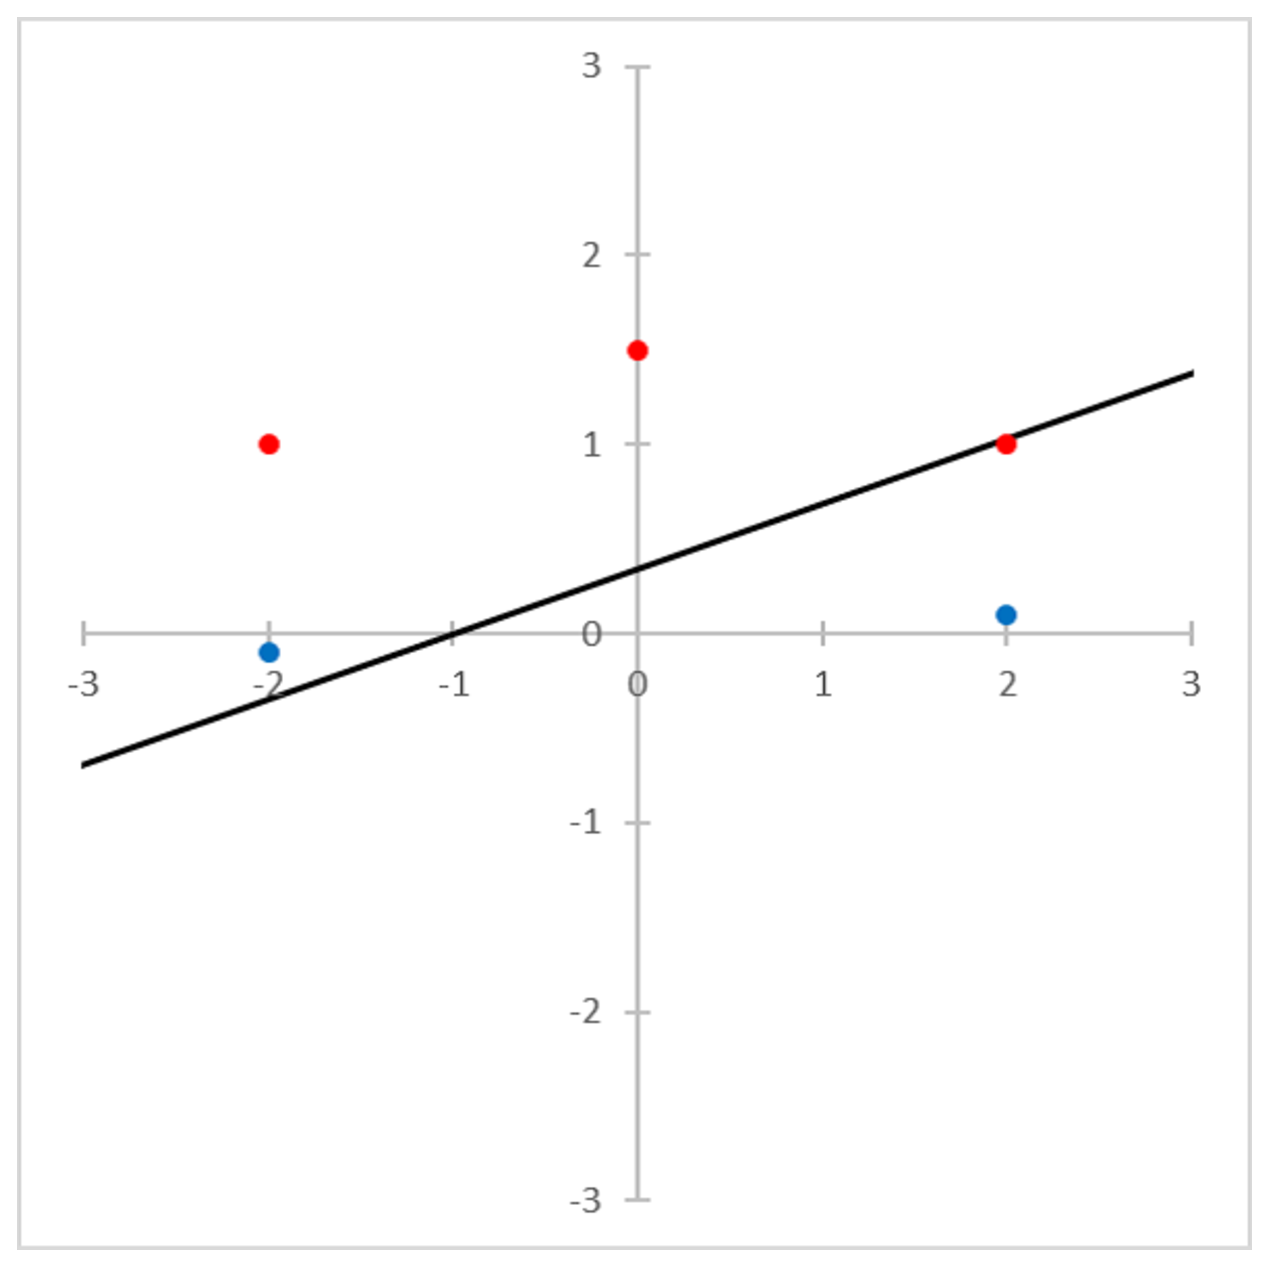
\includegraphics[width=40mm]{./figures/section_2/image5.eps}
            \captionsetup{labelformat=empty,labelsep=none}
            \caption{$w_{(5)}$}
        \end{center}
    \end{minipage}
\end{figure}
\begin{figure}[H]
    \begin{minipage}{0.3\hsize}
        \begin{center}
            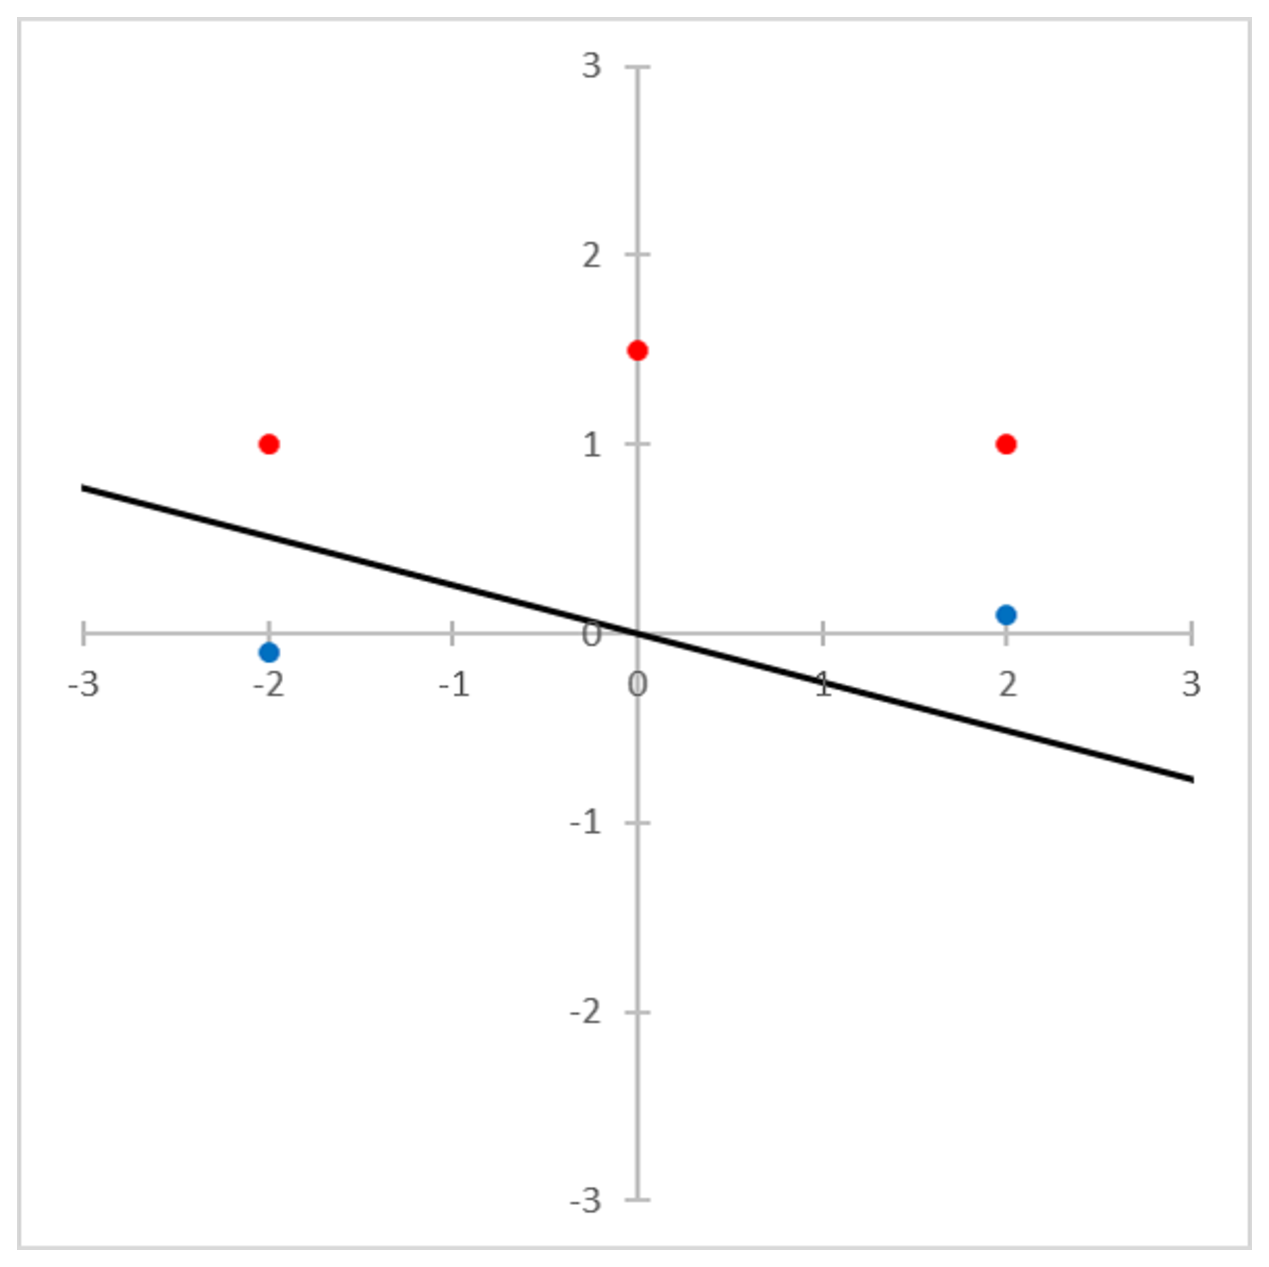
\includegraphics[width=40mm]{./figures/section_2/image6.eps}
            \captionsetup{labelformat=empty,labelsep=none}
            \caption{$w_{(6)}$}
        \end{center}
    \end{minipage}
    \begin{minipage}{0.3\hsize}
        \begin{center}
            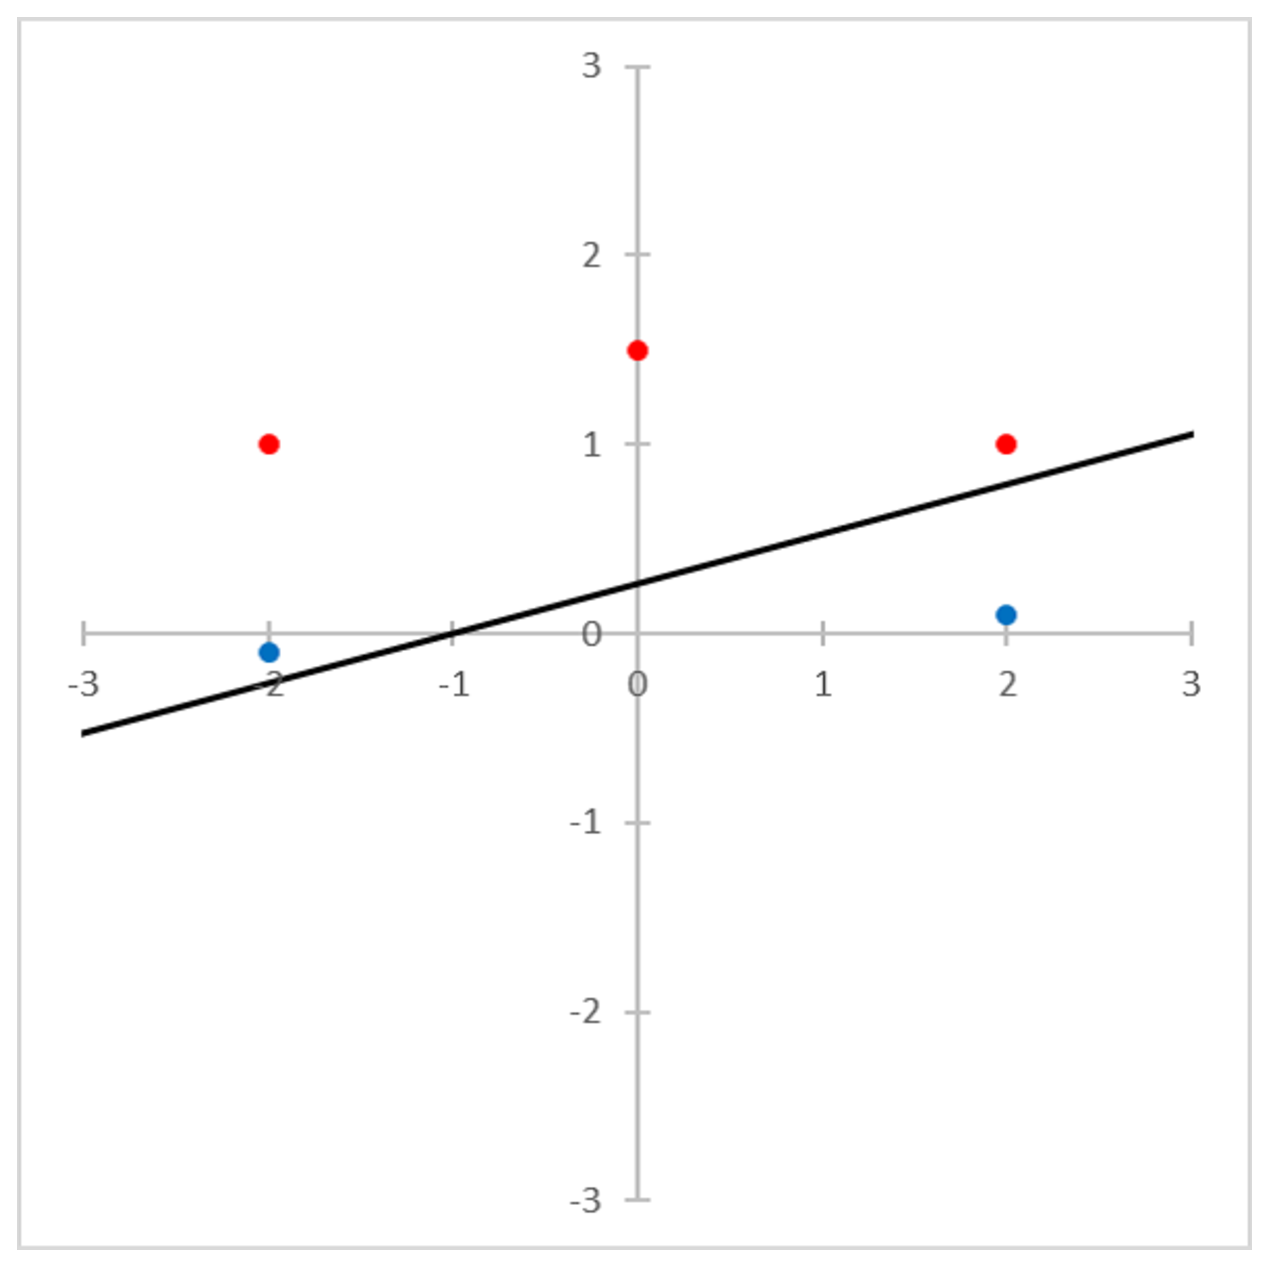
\includegraphics[width=40mm]{./figures/section_2/image7.eps}
            \captionsetup{labelformat=empty,labelsep=none}
            \caption{$w_{(7)}$}
        \end{center}
    \end{minipage}
    \begin{minipage}{0.3\hsize}
        \begin{center}
            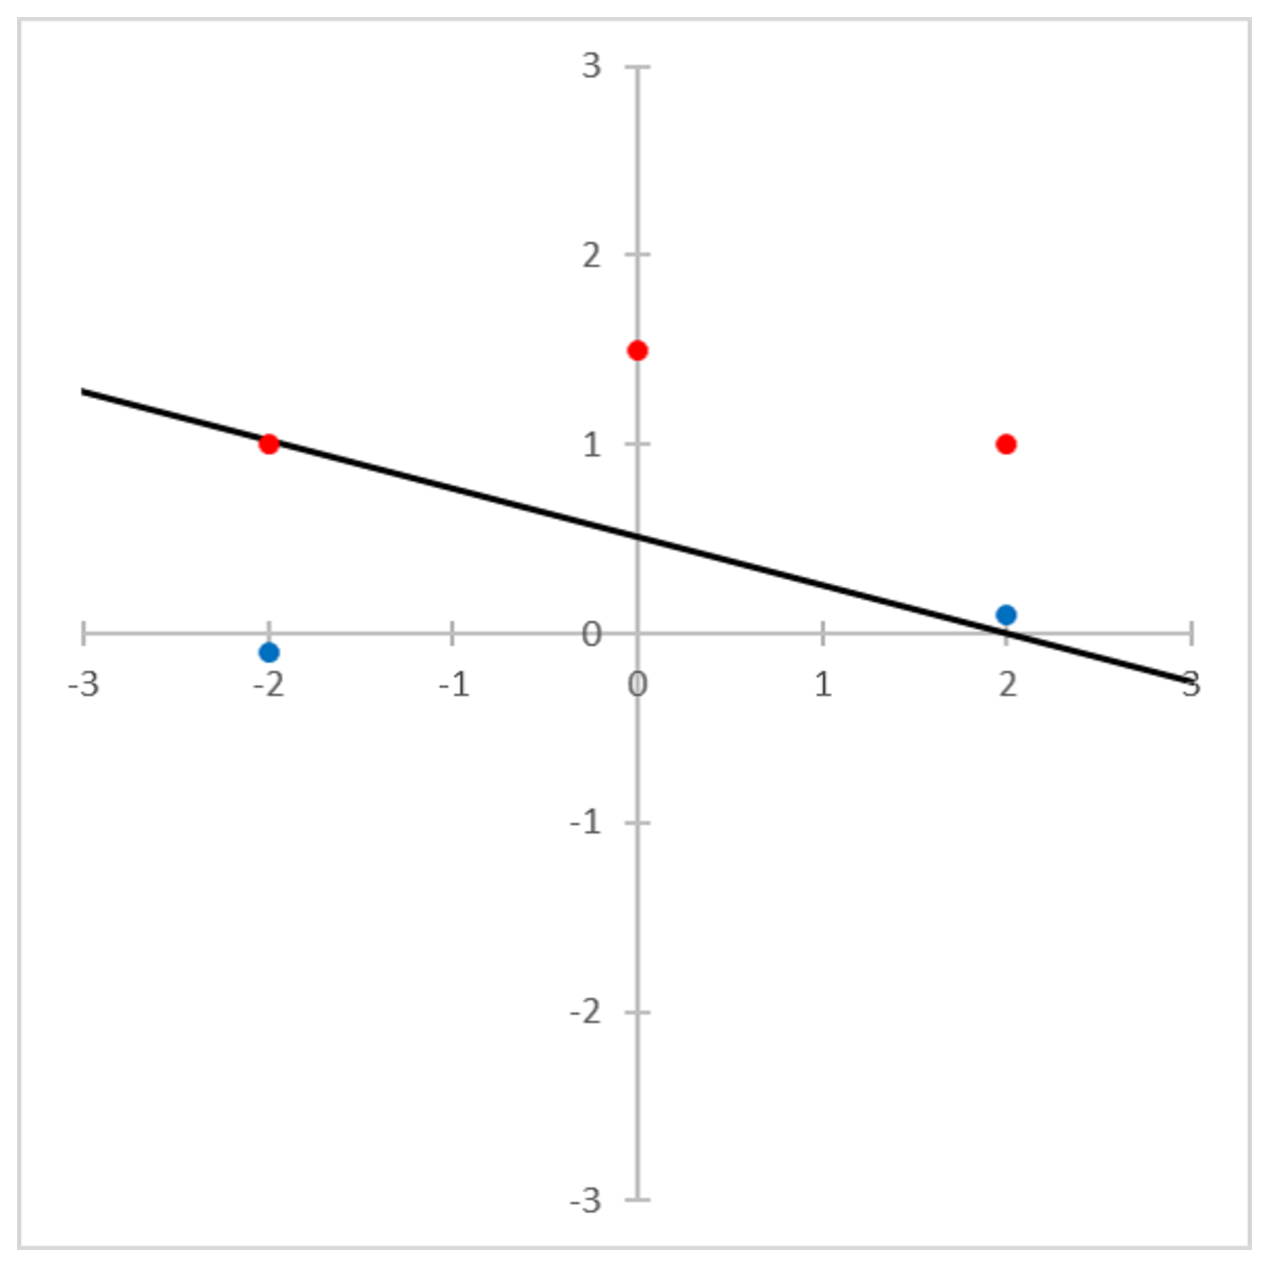
\includegraphics[width=40mm]{./figures/section_2/image8.eps}
            \captionsetup{labelformat=empty,labelsep=none}
            \caption{$w_{(8)}$}
        \end{center}
    \end{minipage}
\end{figure}
\begin{figure}[H]
    \begin{minipage}{0.3\hsize}
        \begin{center}
            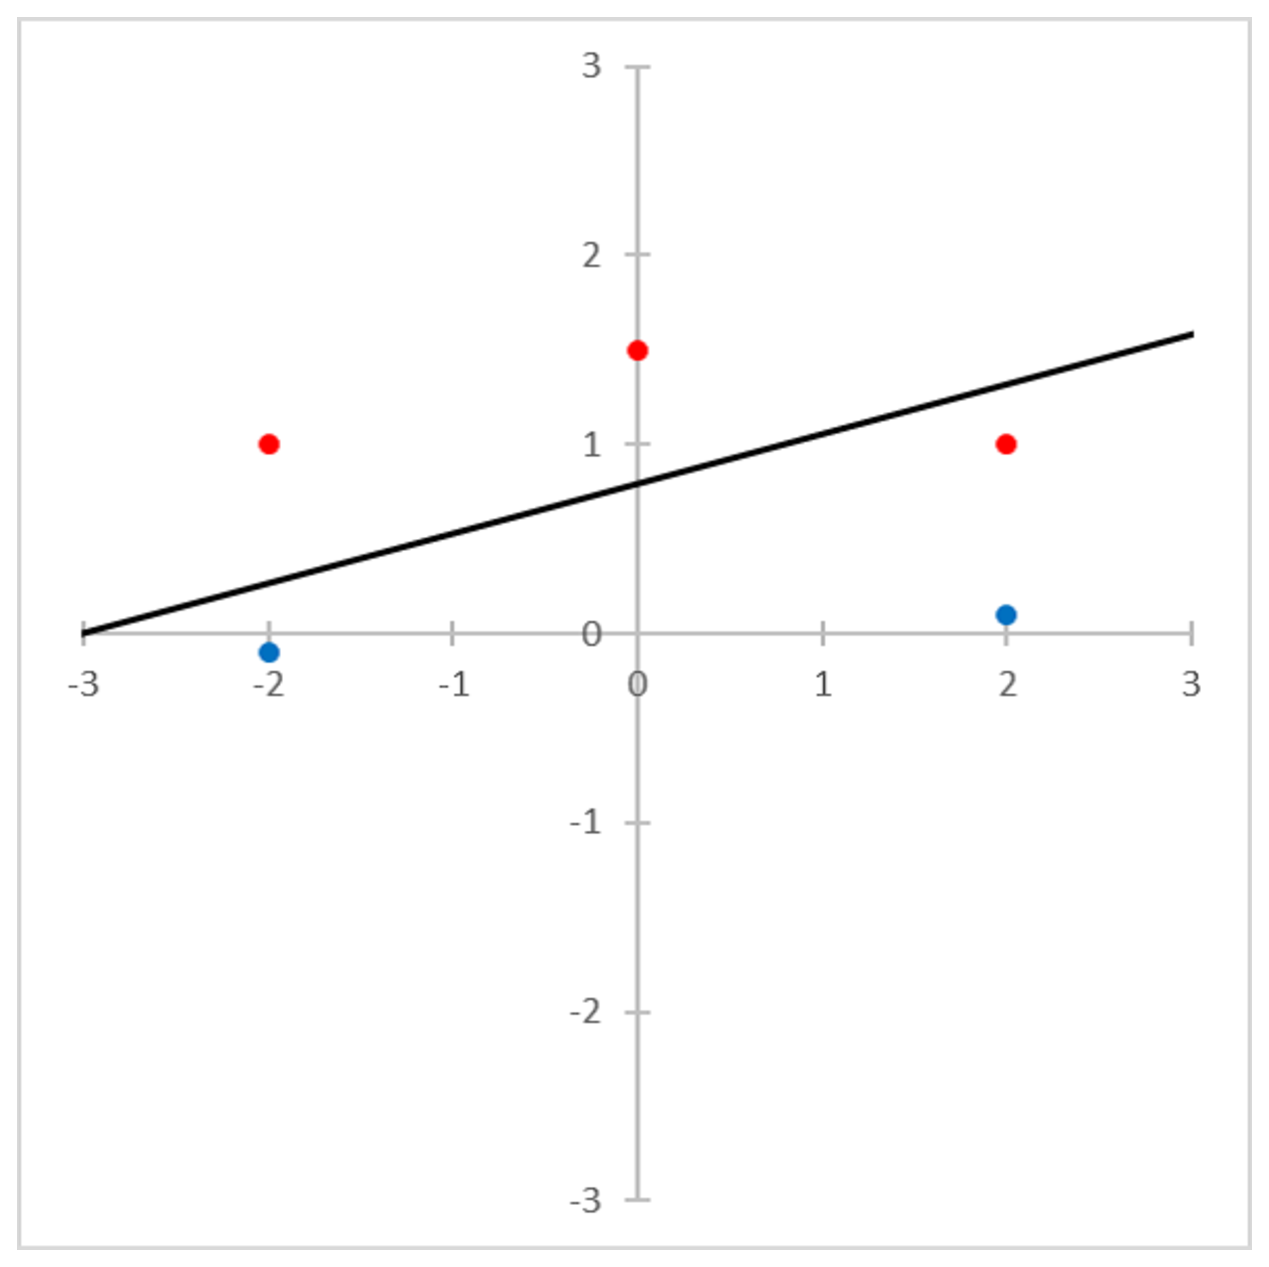
\includegraphics[width=40mm]{./figures/section_2/image9.eps}
            \captionsetup{labelformat=empty,labelsep=none}
            \caption{$w_{(9)}$}
        \end{center}
    \end{minipage}
    \begin{minipage}{0.3\hsize}
        \begin{center}
            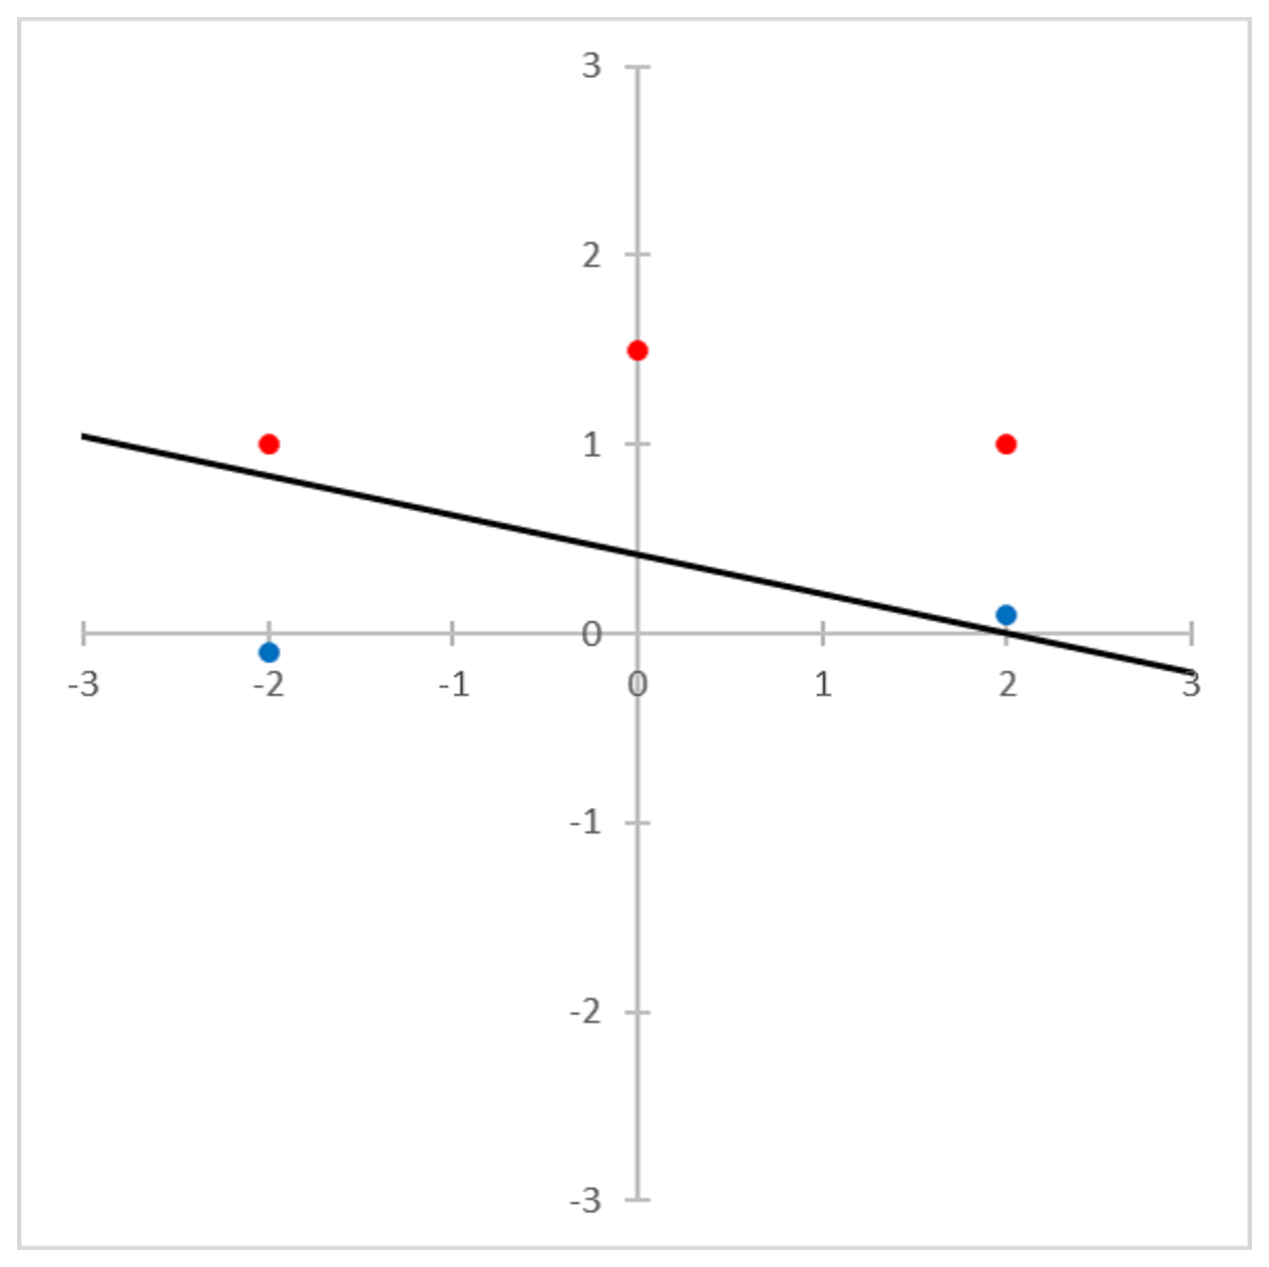
\includegraphics[width=40mm]{./figures/section_2/image10.eps}
            \captionsetup{labelformat=empty,labelsep=none}
            \caption{$w_{(10)}$}
        \end{center}
    \end{minipage}
    \begin{minipage}{0.3\hsize}
        \begin{center}
            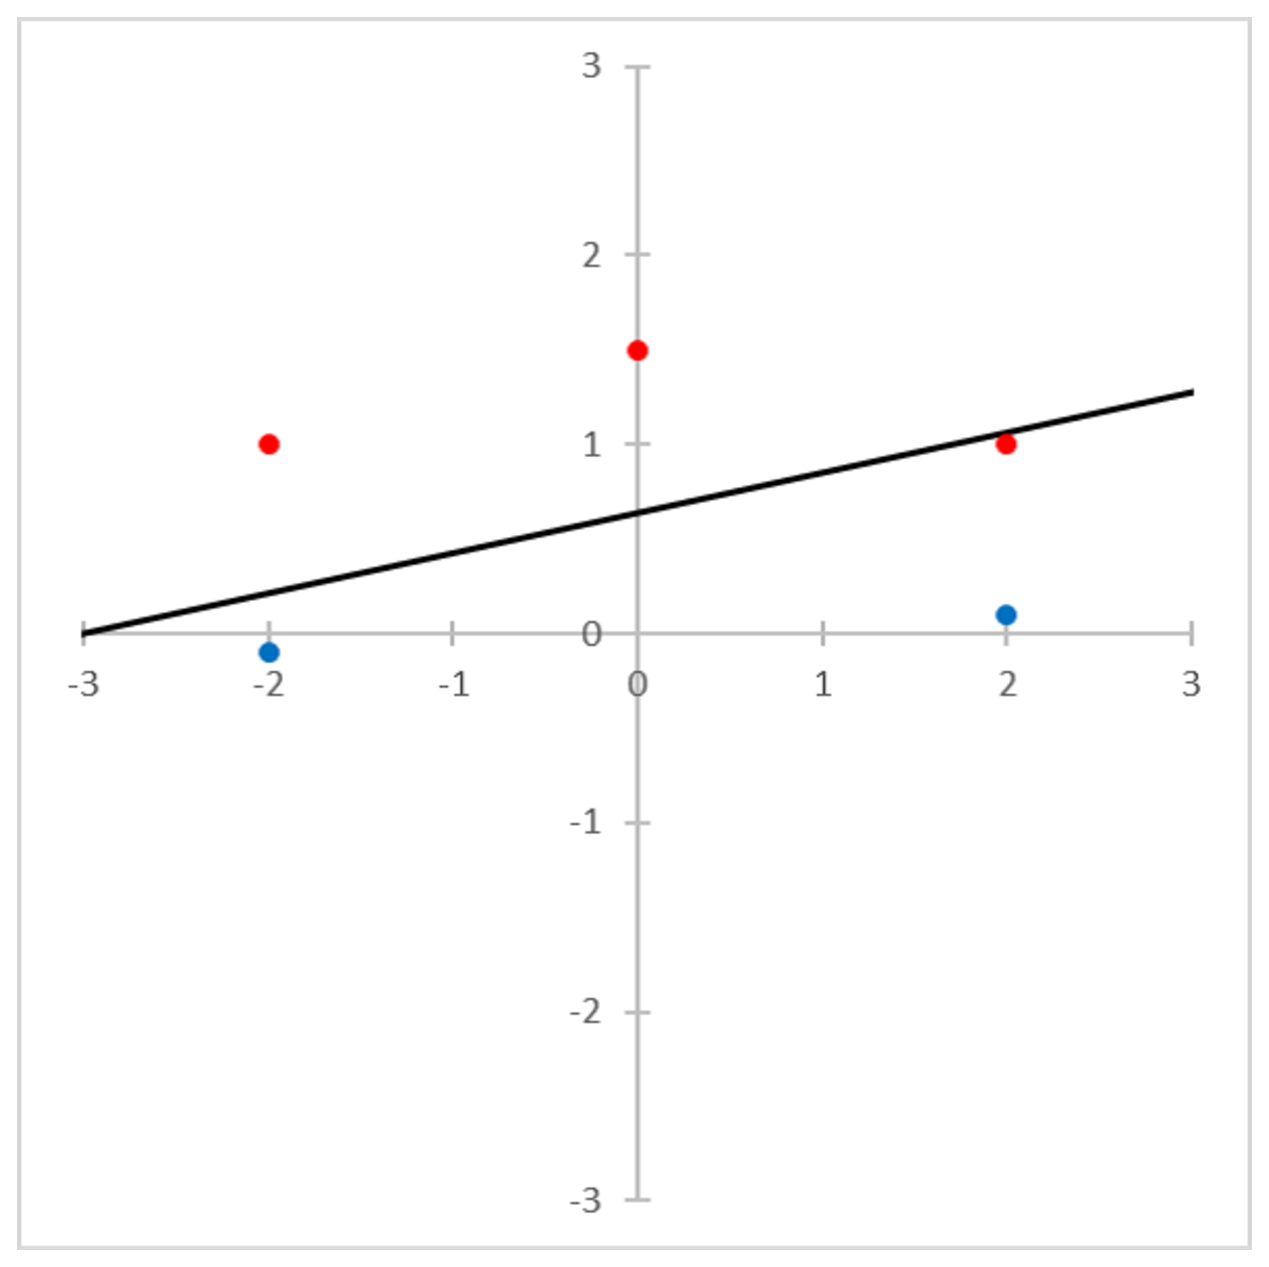
\includegraphics[width=40mm]{./figures/section_2/image11.eps}
            \captionsetup{labelformat=empty,labelsep=none}
            \caption{$w_{(11)}$}
        \end{center}
    \end{minipage}
\end{figure}
\begin{figure}[H]
    \begin{minipage}{0.3\hsize}
        \begin{center}
            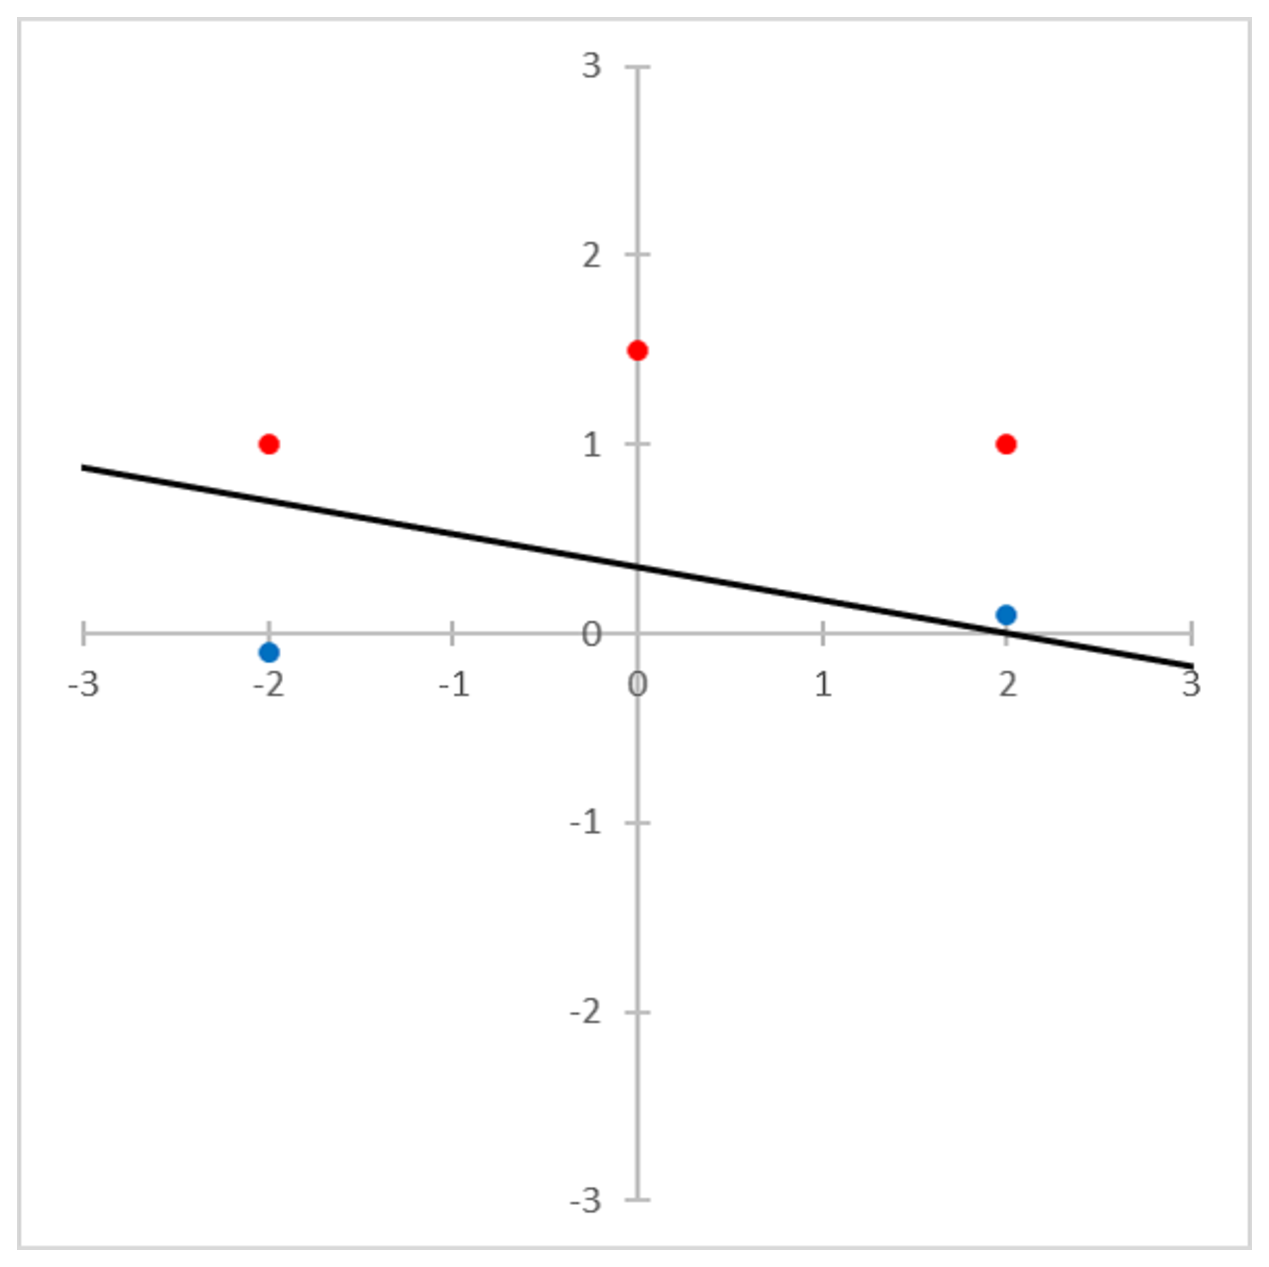
\includegraphics[width=40mm]{./figures/section_2/image12.eps}
            \captionsetup{labelformat=empty,labelsep=none}
            \caption{$w_{(12)}$}
        \end{center}
    \end{minipage}
    \begin{minipage}{0.3\hsize}
        \begin{center}
            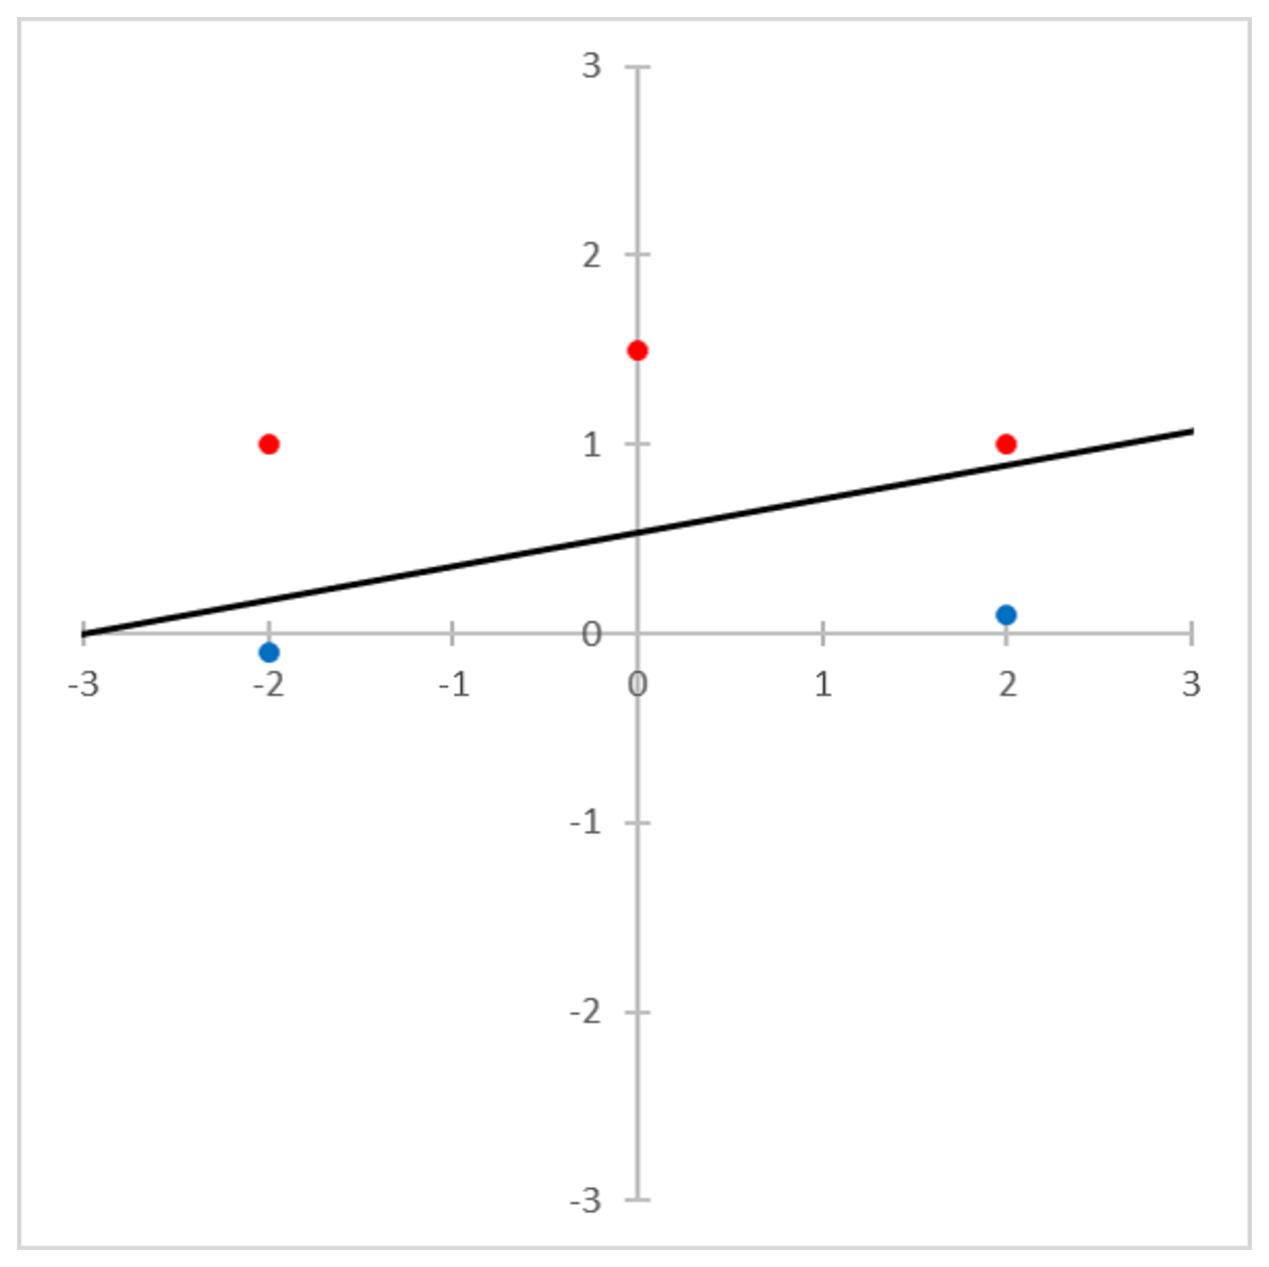
\includegraphics[width=40mm]{./figures/section_2/image13.eps}
            \captionsetup{labelformat=empty,labelsep=none}
            \caption{$w_{(13)}$}
        \end{center}
    \end{minipage}
\end{figure}
\section*{問題3}
\noindent
原点中心の単位円より
\begin{eqnarray*}
    x_1^2+x_2^2=1
\end{eqnarray*}
となればよい\\
また,モデルの式から
\begin{eqnarray*}
    w_1f_1(x_1)+w_2f_2(x_2)-w_0=0\\
    w_1f_1(x_1)+w_2f_2(x_2)=w_0
\end{eqnarray*}
両辺を$w_0$で割って
\begin{eqnarray*}
    \frac{w_1}{w_0}f_1(x_1)+\frac{w_2}{w_0}f_2(x_2)=1
\end{eqnarray*}
となる\\
よって,最初の式と比較すると
\begin{eqnarray*}
    \left\{\begin{array}{c}f_1(x_1)=\frac{w_0}{w_1}x_1^2\\\\f_2(x_2)=\frac{w_0}{w_2}x_2^2\end{array}\right.
\end{eqnarray*}
と定義すれば,原点中心の単位円の識別が可能となる.

\end{document}